\documentclass{article}

\usepackage{tikz}
\usepackage{amsmath}
\usepackage[left=2.3cm, right=2.3cm, top=1.7cm, bottom=1.7cm]{geometry}

\usepackage{Sweave}
\begin{document}
\input{test-concordance}

{\Large \textbf{Name:} \hspace{3cm} \vspace{1cm}

\begin{center}
{\Huge Stage 1 - General Maths Networks Test}
\end{center}
\vspace{0.2cm}


%%%%%%%%%%%%%%%%%%%%%%
%%%   Question 1   %%%
%%%%%%%%%%%%%%%%%%%%%%
\vspace{0.2cm}
\hspace{1cm}
\textbf{Question 1} 

\vspace{0.5cm}
\begin{center}
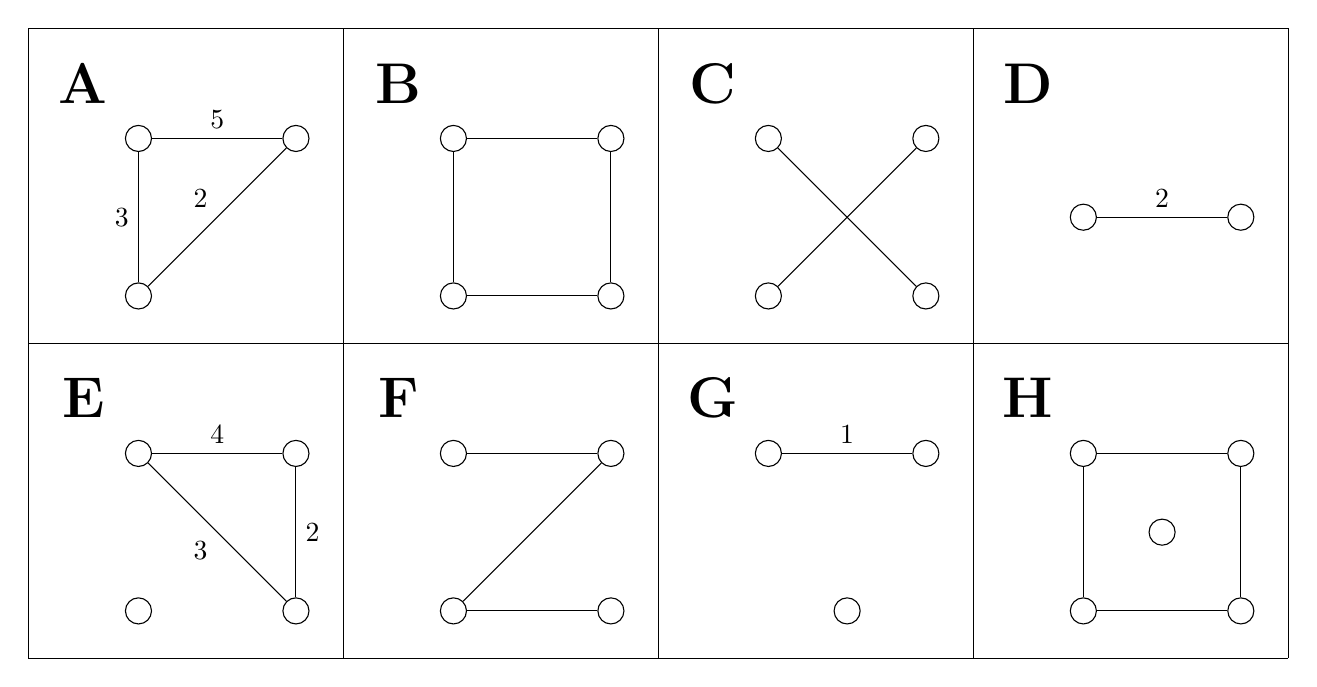
\begin{tikzpicture}
  \draw (-0.7, 6.7) node {\huge \textbf{A}};
  \node[draw=black, circle] (a) at (0,6) {};
  \node[draw=black, circle] (b) at (2,6) {};
  \node[draw=black, circle] (c) at (0,4) {};
  \draw (a) -- node[above] {5} ++(b);
  \draw (a) -- node[left] {3} ++(c);
  \draw (b) -- node[above left] {2} ++(c);

  \draw (3.3, 6.7) node {\huge \textbf{B}};
  \node[draw=black, circle] (a) at (4,6) {};
  \node[draw=black, circle] (b) at (6,6) {};
  \node[draw=black, circle] (c) at (4,4) {};
  \node[draw=black, circle] (d) at (6,4) {};
  \draw (a) -- (b);
  \draw (a) -- (c);
  \draw (b) -- (d);
  \draw (c) -- (d);

  \draw (7.3, 6.7) node {\huge \textbf{C}};
  \node[draw=black, circle] (a) at (8,6) {};
  \node[draw=black, circle] (b) at (10,6) {};
  \node[draw=black, circle] (c) at (8,4) {};
  \node[draw=black, circle] (d) at (10,4) {};
  \draw (a) -- (d);
  \draw (b) -- (c);

  \draw (11.3, 6.7) node {\huge \textbf{D}};
  \node[draw=black, circle] (a) at (12,5) {};
  \node[draw=black, circle] (b) at (14,5) {};
  \draw (a) -- node[above] {2} ++(b);

  \draw (-0.7, 2.7) node {\huge \textbf{E}};
  \node[draw=black, circle] (a) at (0,2) {};
  \node[draw=black, circle] (b) at (2,2) {};
  \node[draw=black, circle] (c) at (0,0) {};
  \node[draw=black, circle] (d) at (2,0) {};
  \draw (a) -- node[above] {4} ++(b);
  \draw (a) -- node[below left] {3} ++(d);
  \draw (b) -- node[right] {2} ++(d);

  \draw (3.3, 2.7) node {\huge \textbf{F}};
  \node[draw=black, circle] (a) at (4,2) {};
  \node[draw=black, circle] (b) at (6,2) {};
  \node[draw=black, circle] (c) at (4,0) {};
  \node[draw=black, circle] (d) at (6,0) {};
  \draw (a) -- (b);
  \draw (b) -- (c);
  \draw (c) -- (d);

  \draw (7.3, 2.7) node {\huge \textbf{G}};
  \node[draw=black, circle] (a) at (8,2) {};
  \node[draw=black, circle] (b) at (10,2) {};
  \node[draw=black, circle] (c) at (9,0) {};
  \draw (a) -- node[above] {1} ++(b);

  \draw (11.3, 2.7) node {\huge \textbf{H}};
  \node[draw=black, circle] (a) at (12,2) {};
  \node[draw=black, circle] (b) at (14,2) {};
  \node[draw=black, circle] (c) at (13,1) {};
  \node[draw=black, circle] (d) at (12,0) {};
  \node[draw=black, circle] (e) at (14,0) {};
  \draw (a) -- (b);
  \draw (a) -- (d);
  \draw (b) -- (e);
  \draw (d) -- (e);

  \draw (-1.4,-0.6) -- (14.6,-0.6);
  \draw (-1.4,3.4) -- (14.6,3.4);
  \draw (-1.4,7.4) -- (14.6,7.4);
  
  \draw (-1.4,-0.6) -- (-1.4,7.4);
  \draw (2.6,-0.6) -- (2.6,7.4);
  \draw (6.6,-0.6) -- (6.6,7.4);
  \draw (10.6,-0.6) -- (10.6,7.4);
  \draw (14.6,-0.6) -- (14.6,7.4);

\end{tikzpicture}
\end{center}
\vspace{0.2cm}

By considering the networks above, complete the table below.
\vspace{0.2cm}

\begin{center}
\begin{tabular}{|c|p{2cm}|p{2cm}|p{2.5cm}|p{2.5cm}|p{2.55cm}|}
\hline
Network & Number of Nodes & Number of Edges & Connected Network (Yes or No)  & Weighted Network (Yes or No) & Contains a Circuit (Yes or No) \\ \hline
A & & & & & \\ \hline
B & & & & & \\ \hline
C & & & & & \\ \hline
D & & & & & \\ \hline
E & & & & & \\ \hline
F & & & & & \\ \hline
G & & & & & \\ \hline
\end{tabular}
\end{center}






%%%%%%%%%%%%%%%%%%%%%%
%%%   Question 2   %%%
%%%%%%%%%%%%%%%%%%%%%%
\pagebreak
\hspace{1cm}
\textbf{Question 2} 

\vspace{0.5cm}
\begin{center}
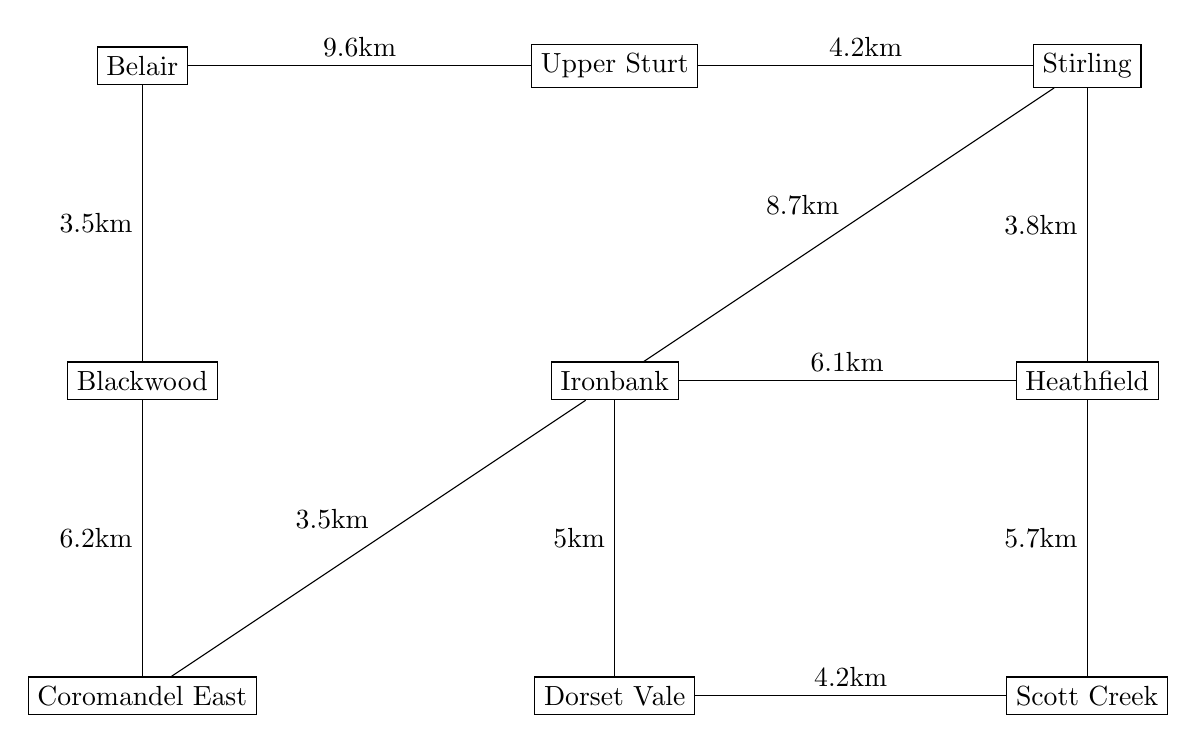
\begin{tikzpicture}
  \node[draw=black] (a) at (0,4) {Blackwood};
  \node[draw=black] (b) at (0,8) {Belair};  
  \node[draw=black] (c) at (0,0) {Coromandel East};  
  \node[draw=black] (d) at (6,4) {Ironbank};  
  \node[draw=black] (e) at (6,8) {Upper Sturt};  
  \node[draw=black] (f) at (12,8) {Stirling};  
  \node[draw=black] (g) at (12,4) {Heathfield};  
  \node[draw=black] (h) at (12,0) {Scott Creek};  
  \node[draw=black] (i) at (6,0) {Dorset Vale};  

  \draw (a) -- node[left] {3.5km} ++(b);
  \draw (a) -- node[left] {6.2km} ++(c);
  \draw (b) -- node[above] {9.6km} ++(e);
  \draw (c) -- node[above left] {3.5km} ++(d);
  \draw (d) -- node[above left] {8.7km} ++(f);
  \draw (d) -- node[above] {6.1km} ++(g);
  \draw (d) -- node[left] {5km} ++(i);
  \draw (e) -- node[above] {4.2km} ++(f);
  \draw (f) -- node[left] {3.8km} ++(g);
  \draw (g) -- node[left] {5.7km} ++(h);
  \draw (h) -- node[above] {4.2km} ++(i);
\end{tikzpicture}
\end{center}
\vspace{0.2cm}

\textbf{(a)} What is represented by the nodes in the networks above?

\vspace{0.6cm}
\begin{center}
\begin{tikzpicture}[scale=0.8]
\draw[black,thin] (0,0) -- (20, 0);
\draw[black,thin] (0,1.5) -- (20, 1.5);
\end{tikzpicture}
\end{center}


\textbf{(b)} What is represented by the edges in the networks above?

\vspace{0.6cm}
\begin{center}
\begin{tikzpicture}[scale=0.8]
\draw[black,thin] (0,0) -- (20, 0);
\draw[black,thin] (0,1.5) -- (20, 1.5);
\end{tikzpicture}
\end{center}

\pagebreak
\textbf{(c)} Apply both Prim's and Kruskal's algorithms in order to find a minimum spanning tree and highlight the edges in this minimum spanning tree in the network diagram above. 
\vspace{10cm}

\textbf{(d)} Describe the difference between Prim's and Kruskal's algorithm in terms of the steps you follow to arrive at a minimum spanning tree.

\vspace{0.6cm}
\begin{center}
\begin{tikzpicture}[scale=0.8]
\draw[black,thin] (0,0) -- (20, 0);
\draw[black,thin] (0,1.5) -- (20, 1.5);
\draw[black,thin] (0,3) -- (20, 3);
\draw[black,thin] (0,4.5) -- (20, 4.5);
\draw[black,thin] (0,6) -- (20, 6);
\end{tikzpicture}
\end{center}






%%%%%%%%%%%%%%%%%%%%%%
%%%   Question 3   %%%
%%%%%%%%%%%%%%%%%%%%%%
\pagebreak
\hspace{1cm}
\textbf{Question 3} 

\vspace{0.6cm}
\begin{center}
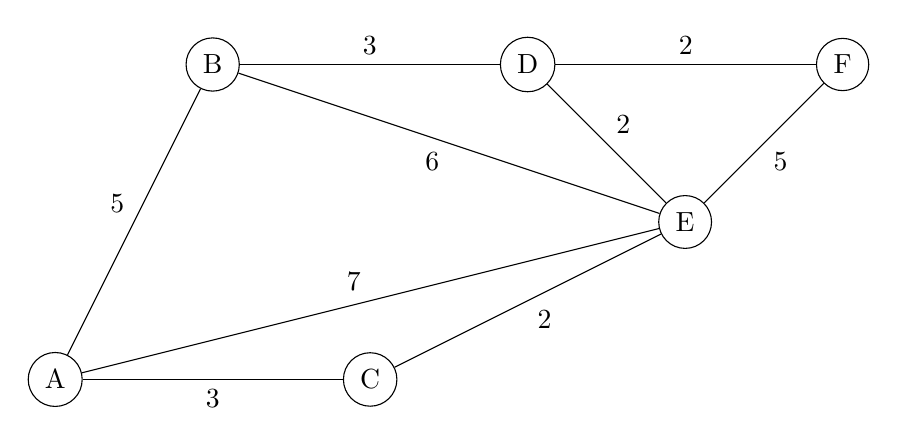
\begin{tikzpicture}
  \node[draw=black, circle] (a) at (0,0) {A};
  \node[draw=black, circle] (b) at (2,4) {B};  
  \node[draw=black, circle] (c) at (4,0) {C};  
  \node[draw=black, circle] (d) at (6,4) {D};  
  \node[draw=black, circle] (e) at (8,2) {E};  
  \node[draw=black, circle] (f) at (10,4) {F};  

  \draw (a) -- node[above left] {5} ++(b);
  \draw (a) -- node[below] {3} ++(c);
  \draw (a) -- node[above left] {7} ++(e);
  \draw (b) -- node[above] {3} ++(d);
  \draw (b) -- node[below left] {6} ++(e);
  \draw (c) -- node[below right] {2} ++(e);
  \draw (d) -- node[above right] {2} ++(e);
  \draw (d) -- node[above] {2} ++(f);
  \draw (e) -- node[below right] {5} ++(f);
\end{tikzpicture}
\end{center}
\vspace{0.2cm}

\textbf{(a)} Use Dijkstra's Algorithm to find the shortest path from A to F in the network shown. Make sure to annotate and box each node appropriately, and neatly cross out labels as needed. Then, write the shortest path here in the form A $\rightarrow \hdots \rightarrow \hdots \rightarrow$ F.
\vspace{0.2cm}

\vspace{0.9cm}
\begin{center}
\begin{tikzpicture}[scale=0.8]
\draw[black,thin] (0,0) -- (20, 0);
\end{tikzpicture}
\end{center}
\vspace{0.2cm}

\textbf{(b)} What is the length of the shortest path you found in (a)? 

\vspace{0.9cm}
\begin{center}
\begin{tikzpicture}[scale=0.8]
\draw[black,thin] (0,0) -- (20, 0);
\end{tikzpicture}
\end{center}
\vspace{0.2cm}

\textbf{(c)} Find the \textbf{longest path} (that does not go through any node more than once) from A to F in the network above. Write the longest path in the form A $\rightarrow \hdots \rightarrow \hdots \rightarrow$ F.
\vspace{0.2cm}

\vspace{0.9cm}
\begin{center}
\begin{tikzpicture}[scale=0.8]
\draw[black,thin] (0,0) -- (20, 0);
\end{tikzpicture}
\end{center}
\vspace{0.2cm}

\textbf{(d)} What is the length of the longest path you found in (c)? 

\vspace{0.9cm}
\begin{center}
\begin{tikzpicture}[scale=0.8]
\draw[black,thin] (0,0) -- (20, 0);
\end{tikzpicture}
\end{center}
\vspace{0.2cm}


\end{document}
